\documentclass[a4paper,twoside]{report}
\usepackage{geometry}
\usepackage{doc}
\usepackage[latin1]{inputenc}
\usepackage[catalan]{babel}
\usepackage{amsfonts}
\usepackage{amsmath}
\usepackage[pdftex]{graphicx}
\usepackage{listings}
\usepackage{fancyhdr}
\usepackage{fancyvrb}
\usepackage{url} 
\usepackage{color}
\usepackage{lscape}
\usepackage{setspace}
\usepackage{float}
\usepackage{longtable}

\usepackage[pdfauthor={Ramon Xuriguera Albareda},%
		pdfsubject={BibTeX Bibliography Index Maker},%
		pdftitle={BibTeX Bibliography Index Maker},%
		pdftex]{hyperref}


\lstset{%
    numbers=none,               %
    breaklines=true,            %
    fancyvrb=false,             %
    tabsize=2,                  % sets default tabsize to 2 spaces
    captionpos=b,               % sets the caption-position to bottom
    frame=single,
    xleftmargin=3em,
    xrightmargin=3em,
    backgroundcolor = \color{lightgrey}
}        
\renewcommand{\lstlistingname}{Llistat}

\newcommand{\tab}{\hspace*{2em}}


\title{\BibTeX{} Bibliography Index Maker: Meeting Notes}
\author{Ramon Xuriguera}
\date{Primavera 2010}

\setlength{\parindent}{0in}
\definecolor{lightgrey}{gray}{0.85}

%%% PAGE STYLE %%%
\pagestyle{fancy}
\fancyhf{}
\renewcommand{\headrulewidth}{0pt}
\renewcommand{\footrulewidth}{0pt}
\fancyhead[LE]{\textit{\nouppercase{\leftmark}}}
\fancyhead[RO]{\textit{\nouppercase{\rightmark}}}
\fancyfoot[C]{\thepage}
 
\fancypagestyle{plain}{ %
\fancyhf{}
}

\setlength{\headheight}{14pt}


\begin{document}
\begin{titlepage}
%\thispagestyle{empty}
\vspace*{52mm}
\hspace{45mm}
\begin{minipage}{112mm}
\textbf{\textit{T�tol:} \BibTeX{} Bibliography Index Maker}\\

\textbf{\textit{Volum:} 1/1}\\
\textbf{\textit{Alumne:} Ramon Xuriguera Albareda}\\

\textbf{\textit{Director/Ponent:} Marta Arias}\\
\textbf{\textit{Departament:} LSI}\\
\textbf{\textit{Data:} Primavera 2010}\\
\end{minipage}

\end{titlepage}

\input{blank}
\thispagestyle{empty}
\begin{doublespace}
\hrule
\vspace{5 mm}
\textbf{DADES DEL PROJECTE}
\\
\\
\textit{T�tol del Projecte:}
\\
\\
\textit{Nom de l'estudiant:} Ramon Xuriguera Albareda\\
\textit{Titulaci�:} Enginyeria Inform�tica\\
\textit{Cr�dits:} 37,5\\
\textit{Director/Ponent:} Marta Arias Vicente\\
\textit{Departament:} LSI\\
\\
\hrule
\vspace{5 mm}
\textbf{MEMBRES DEL TRIBUNAL} \textit{(nom i signatura)}\\
\\
\textit{President:}
\\
\\
\textit{Vocal:}
\\
\\
\textit{Secretari:}
\\
\\
\hrule
\vspace{5 mm}
\textbf{QUALIFICACI�}
\\
\\
\textit{Qualificaci� num�rica:}\\
\textit{Qualificaci� descriptiva:}
\\
\\
\textit{Data:}\\
\hrule
\end{doublespace}

\input{blank}

\begin{abstract}
En aquest document es presenta una aplicaci� que facilita la generaci� autom�tica d'�ndexs bibliogr�fics en format BibTeX a partir de col�leccions d'articles cient�fics en PDF. Aquesta �s una tasca que han dur a terme les persones que realitzen treballs de recerca per aix� poder incloure refer�ncies a altres documents dins de les seves publicacions, un proc�s pesat, repetitiu i que, si s'ha de fer manualment, requereix molt de temps. S'ha dividit la feina en tres grans parts: la cerca a les biblioteques digitals per trobar refer�ncies dels articles, l'extracci� d'informaci� estructurada de p�gines HTML i la creaci� d'aquestes regles d'extracci� fent servir exemples.
\end{abstract}
\input{blank}
\input{blank}
\tableofcontents

\chapter{Introducci�}
\label{chapter:introduction}

El format PDF ha esdevingut un est�ndar per la divulgaci� de publicacions on-line.

\paragraph{}
Actualment existeixen serveis com ara \textit{Google Scholar}, \textit{Microsoft Academic Search} o \textit{CiteSeer} que es dediquen a recol�lectar informaci� sobre articles i que comptabilitzen les refer�ncies entre diferents publicacions. En el cas de \textit{CiteSeer}, al ser un projecte lliure, sabem que funciona analitzant les diferents parts dels articles, com ara les cites,  per� que tamb� t� problemes per obtenir els camps de la cap�alera, que �s el que ens interessa \cite{Giles98citeseer}.

\paragraph{}
Per una altra banda, tamb� existeixen nombroses aplicacions dedicades al maneig de refer�ncies com \textit{\href{http://jabref.sourceforge.net/}{JabRef}}\footnote{\href{http://jabref.sourceforge.net/}{http://jabref.sourceforge.net}} o \textit{\href{http://www.mendeley.com/}{Mendeley}}\footnote{\href{http://www.mendeley.com/}{http://www.mendeley.com}}. Entre algunes de les funcionalitats addicionals que ofereixen, hi ha la possibilitat de cercar en bases de dades d'articles i utilitzar les meta-dades dels fitxers per tal de trobar informaci� com ara el t�tol o l'autor. A banda d'aix�, no n'hem trobat cap que aprofiti el contingut dels documents per generar la refer�ncia.

El nostre sistema mira d'omplir el buit que queda entre aquestes dos tipus de programari que 


\textit{\BibTeX{} Bibliography Index Maker} �s una eina d'ajuda a la creaci� d'�ndexs bibliogr�fics pensada com un complement a aplicacions de maneig de refer�ncies ja existents com poden ser .



\paragraph{}
La principal funcionalitat que ofereix consisteix en escanejar un directori que cont� articles cient�fics en PDF i generar un �ndex bibliogr�fic en \BibTeX{} amb les refer�ncies d'aquests fitxers. Aquest �ndex es pot importar des de les aplicacions esmentades o b� pot ser referenciat directament des d'un nou document \TeX.


Compta amb tres parts principals:

\section{Estructura d'aquest document}
La mem�ria est� dividida en els set cap�tols seg�ents:

\begin{itemize}
\item{Capitol \ref{chapter:definition}:}
Descripci� formal del projecte aix� com un rep�s sobre el disseny.

\item{Capitol \ref{chapter:search}:}
Parla de les t�cniques que s'utilitzen per poder aconseguir p�gines que continguin informaci� sobre els do

\item{Capitol \ref{chapter:refextraction}:}
Tracta sobre com extreure la informaci� sobre els articles de les p�gines d'Internet que hem obtingut.

\item{Capitol \ref{chapter:wrapperinduction}:}
Est� dedicat a les t�cniques per generar, de forma autom�tica, les regles d'extracci� de les refer�ncies.

\item{Capitol \ref{chapter:results}:}
Plantejament de les proves per cadascuna de les parts m�s importants del sistema i an�lisi dels resultats obtinguts.

\end{itemize}

Pel que fa al contingut de les diferents seccions, ens hem volgut centrar, sobretot, en el que fa a les decisions que hem hagut de prendre al llarg de la realitzaci� del projecte i no tant en els aspectes t�cnics de com s'ha implementat el sistema. Per cada decisi� es presenten algunes de les opcions plantejades en un principi, els problemes que aquestes presenten i es passa a descriure la soluci� escollida i els motius de l'elecci�.

\paragraph{}
S'assumeix que es tenen nocions b�siques de l'estructura dels documents HTML i d'expressions regulars, dos temes que no es tractaran. Pel que fa a les expressions regulars, s'utilitzen les operacions que ofereix el m�dul \texttt{re} de \textit{Python}. Es pot trobar m�s informaci� a \cite{pyRegex}.


\chapter{Definici� del Projecte}
\label{chapter:definition}

En aquest segon cap�tol es descriuen les l�nies generals que s'han seguit per dur a terme el projecte i per definir-ne el context. Comencem explicant el procediment que ens permetr� aconseguir els objectius proposats.

\section{Proc�s d'extracci�}
En un principi, la idea que vam plantejar per resoldre el problema de l'extracci� de refer�ncies d'un document PDF va ser intentar distingir la informaci� de la refer�ncia bibliogr�fica directament del fitxer, seguint uns passos semblants als de la figura seg�ent.

\begin{figure}[H]
\begin{center}
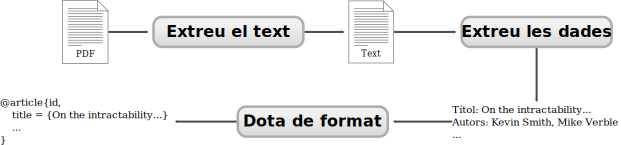
\includegraphics[width=\textwidth]{figures/definition:invalid-extraction-diagram.pdf}
\caption{Primera idea per l'extracci� de refer�ncies}
\label{fig:definition:invalid-extraction-diagram}
\end{center}
\end{figure}

Aix� presenta moltes limitacions. Per comen�ar, la impossibilitat d'extreure informaci� que no es troba dins del text (e.g. el n�mero de p�gines de l'article). A m�s, el text que dels fitxers PDF no t� una estructura prou clara com per poder distingir entre els diferents camp. Aquest segon problema es tracta amb m�s en detall al proper cap�tol.

\paragraph{}
La soluci� que hem trobat per poder tirar endavant consisteix en fer �s del que s'anomenem \textit{biblioteques digitals}: grans bases de dades amb informaci� sobre articles i els corresponents fitxers en format digital. A m�s, la majoria d'elles estan indexades pels principals cercadors disponibles a Internet. Els diagrama actualitzat es mostra a la figura \ref{fig:definition:extraction-diagram}. B�sicament, per cada fitxer l'aplicaci�:
\begin{enumerate}
    \item{Extreu el contingut en forma de text.}
    \item{Genera un llistat de consultes a partir del text extret.}
    \item{Obt� els resultats d'aquestes consultes amb algun cercador (Google, Bing, etc.).}
    \item{Mira d'extreure la refer�ncia de les p�gines retornades pel cercador.}
    \item{Comprova que les dades de la refer�ncia corresponen al fitxer.}
    \item{D�na format a les dades de la refer�ncia.}
\end{enumerate}

\begin{figure}[H]
\begin{center}
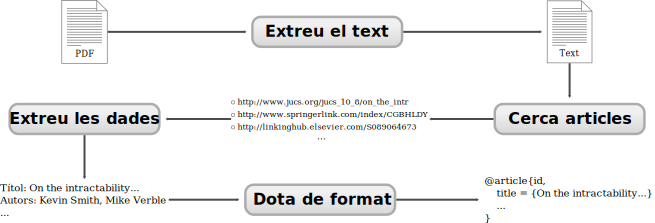
\includegraphics[width=\textwidth]{figures/definition:extraction-diagram.pdf}
\caption{Esquema del proc�s a seguir per extreure una refer�ncia}
\label{fig:definition:extraction-diagram}
\end{center}
\end{figure}

Aix� doncs, hem de fer una mica m�s de tomb per poder aconseguir els resultats desitjats, per� els passos s�n m�s senzills d'aplicar, donant-nos m�s garanties que funcionar�.


\section{\BibTeX}
\label{chapter:definition:section:bibtex}
Per poder entendre el context del projecte cal que descrivim l'eina de maneig de refer�ncies \BibTeX{} i la sintaxi del llenguatge que utilitza. 
En el nostre cas farem servir aquest llenguatge com a format de sortida al generar els �ndexos bibliogr�fics. Al llistat \ref{listing:exampleBibTeX} es mostra un exemple d'una refer�ncia d'un article cient�fic expressat en el format \BibTeX:
\begin{center}
\begin{lstlisting}[caption={Refer�ncia expressada en \BibTeX}, label=listing:exampleBibTeX]
@article{MoSh:27,
  title = {Size direction games over the real line},
  author = {Moran, Gadi and Shelah, M., Saharon},
  journal = {Israel Journal of Mathematics},
  pages = {442--449},
  volume = {14},
  year = {1973},
}
\end{lstlisting}
\end{center}

Alguns aspectes a comentar sobre l'exemple anterior:
\begin{itemize}
\item{}
La primera l�nia cont� el tipus de document i un identificador. El primer defineix els camps obligatoris que s'han d'especificar, i el segon ens permetr� citar a la refer�ncia des d'un document. En el nostre cas nom�s ens interessen les refer�ncies de tipus \textit{article} i haurem de definir, com a m�nim, els camps \textit{author}, \textit{title}, \textit{journal} i \textit{year}, que s�n obligatoris.

\item{}
Es considera que el nom d'un autor o editor pot constar de quatre parts diferents: \textit{First}, \textit{von}, \textit{Last}, \textit{Jr.}. Es poden ordenar de diverses maneres, per� nosaltres ho farem amb \texttt{<von> <last>, <middle>, <first>}. Cal separar m�ltiples noms amb la paraula \texttt{and}.

\item{}
L'�ltim camp d'una refer�ncia pot acabar o no amb una coma.
\end{itemize}

\section{Funcionalitats}
A continuaci� es llisten totes les funcionalitats que l'aplicaci� ofereix a l'usuari final:
\begin{itemize}
\item{}
Extracci� de la refer�ncia bibliogr�fica corresponent a un o m�s articles que es troben en fitxers PDF en algun directori.

\item{}
Possibilitat d'exportar les refer�ncies extretes en format \BibTeX{} i desar-les a un fitxer \texttt{.bib}

\item{}
Generaci� autom�tica de regles d'extracci� a partir d'exemples.

\item{}
Importaci� de refer�ncies en un fitxer \texttt{.bib} per tal de poder-los fer servir d'exemples.

\item{}
Totes les operacions CRUD\footnote{\textit{Create}, \textit{read}, \textit{update} i \textit{delete}.} per a la gesti� de refer�ncies i regles d'extracci�.
\end{itemize}


\section{Disseny del sistema}
Hem organitzat el codi del sistema en els m�duls que es llisten a continuaci�:
\begin{itemize}
\item{\textit{Raw Content Extraction} (rce):}
Agrupa totes les classes encarregades d'extreure el contingut dels documents PDF.

\item{\textit{Information Retrieval} (ir):}
Encarregat de comunicar-se amb els diferents cercadors disponibles a Internet per obtenir p�gines que contenen informaci� de la refer�ncia que volem extreure.

\item{\textit{Information Extraction} (ie):}
Cont� tot el codi que permet obtenir la refer�ncia a partir d'una p�gina HTML. A m�s, tamb� �s l'encarregat de generar nous \textit{wrappers}.

\item{\textit{References}:}
Per una banda fa un an�lisis sint�ctic de les refer�ncies extretes per poder-les validar. Per l'altra, transforma a \BibTeX les refer�ncies extretes.

\item{Base de dades (db):}
Tal i com indica el seu nom, duu a terme els accessos la base de dades.

\item{\textit{Main}: }
Enlla�a tots els m�duls anteriors i proporciona punts d'entrada a la interf�cie d'usuari. Fa de fa�ana del sistema.

\item{\textit{Graphical User Interface} (gui):}
Interf�cie d'usuari m�s o menys amigable.
\end{itemize}

La figura \ref{fig:module_diagram} mostra com interaccionen entre ells.

\begin{figure}[H]
\begin{center}

\includegraphics[width=0.6\textwidth]{figures/module_diagram.pdf}
\caption{M�duls del sistema}
\label{fig:module_diagram}
\end{center}
\end{figure}


\section{Llista de tasques}
A continuaci� es llisten les diferents tasques que s'han dut a terme durant la realitzaci� del projecte:
\begin{center}
\begin{longtable}{|l|}

\hline
\textbf{Tasca}                                                              \\
\hline
\hline
Recerca i proves de concepte                                                \\
Infraestructura (repositori, \textit{build tracker}, etc.)                  \\   

Extracci� del text dels PDF (\texttt{bibim.rce})                            \\
\tab Comparaci� de resultats entre les diferents eines                      \\
\tab Tria de l'eina d'extracci�                                             \\

Obtenci� de p�gines amb la refer�ncia (\texttt{bibim.ir})                   \\
\tab Obtenir consultes del text                                             \\
\tab \textit{Browser} per obtenir p�gines de la Web                         \\
\tab �s de les APIs dels cercadors                                          \\
\tab Cerca de les consultes (m�ltiples cercadors)                           \\
\tab Ordenaci� resultats de la cerca                                        \\   

Extracci� d'informaci� (\texttt{bibim.ie})                                  \\
\tab An�lisi de l'estructura d'algunes biblioteques digitals disponibles    \\
\tab \textit{Wrappers} a m� per extreure refer�ncies directament            \\
\tab \textit{Wrappers} a m� per extreure camps                              \\                    
\tab Validaci� de les refer�ncies extretes                                  \\

Generaci� autom�tica de \textit{wrappers}                                   \\
\tab Extracci� d'exemples                                                   \\
\tab Generaci� de regles                                                    \\
\tab \textit{Wrapper} gen�ric                                               \\
\hline

Tractament de refer�ncies (\texttt{bibim.references})                       \\
\tab \textit{Parsing}                                                       \\
\tab Generaci�                                                              \\
\tab Crear �ndexs                                                           \\




Base de dades (\texttt{bibim.db})                                           \\
\tab Disseny
\tab 

    

M�dul principal (\texttt{bibim.main})                                       \\
\tab Escaneig de fitxers                                                    \\
\tab Codi principal de l'aplicaci�                                          \\
\tab \textit{Threading}                                                     \\
\tab Validaci� de refer�ncies                                               \\
\hline


Interf�cie d'usuari (\texttt{bibim.ui})                                     \\
\tab Editor de refer�ncies                                                  \\
\tab Editor de \textit{wrappers}                                            \\
\hline
\hline
\end{longtable}
\end{center}

\chapter{Cerca de refer�ncies}
\label{chapter:search}

%%%% EXTRACCI� PDF %%%%
\section{Extracci� dels continguts d'un PDF}
El primer pas per poder obtenir la refer�ncia d'un article en un fitxer PDF �s l'extracci� del contingut d'aquest fitxer. Aquest �s un dels aspectes que han influ�t m�s en l'enfocament que hem donat al sistema, pels motius que es descriuen a continuaci�.
\paragraph{}
Tal i com ja hem esmentat, en un principi, la soluci� que es va plantejar era intentar extreure la refer�ncia bibliogr�fica d'un document directament del fitxer PDF del qual es disposa. Tot i les limitacions que aix� suposa, despr�s de veure com queden els articles al convertir-los a text ens vam allunyar encara m�s d'aquesta idea.
\\

\begin{lstlisting}[caption={Text corresponent a la cap�alera d'un article despr�s d'haver-lo extret d'un PDF}, label=listing:examplePDFExtraction01]
Characterization and Armstrong Relations for Degenerate Multivalued Dependencies Using Formal Concept Analysis
Jaume Baixeries and Jos� Luis Balc�zar e a
Dept. Llenguatges i Sistemes Inform`tics, a Universitat Polit`cnica de Catalunya, e c/ Jordi Girona, 1-3, 08034 Barcelona {jbaixer, balqui}@lsi.upc.es

Abstract. Functional dependencies, a notion originated ...
\end{lstlisting}

Els llistats \ref{listing:examplePDFExtraction01} i \ref{listing:examplePDFExtraction02} mostren exemples de les cap�aleres de dos articles diferents despr�s d'haver extret el text del fitxer PDF en el que es trobaven. Com es pot veure, el resultat no t� cap tipus d'estructura que pugui deixar intuir quina part del text correspon a cada fragment d'informaci�, sin� que �s un conglomerat de totes dades. El primer article comen�a amb el t�tol i segueix amb els noms dels dos autors i la informaci� de la universitat. En canvi, el segon comen�a amb l'any, la confer�ncia on s'ha presentat, t�tol i per cada autor es d�na informaci� diferent sobre la universitat. Si comencem a mirar m�s articles, el n�mero de casos amb estructures diferents no para d'augmentar (hi ha m�s exemples a l'ap�ndix \ref{appendix-pdf2text}).
\\

\begin{lstlisting}[caption={Un altre exemple de text extret d'un PDF}, label=listing:examplePDFExtraction02]
2010 Second International Conference on Future Networks

Cloud Computing Research and Development Trend
Shuai Zhang Hebei Polytechnic University College of Science Hebei Polytechnic University NO.46 Xinhua West Street Tangshan 063009, Hebei Province China zhangshuai@heut.edu.cn Xuebin Chen Hebei Polytechnic University College of Science Hebei Polytechnic University NO.46 Xinhua West Street Tangshan 063009, Hebei Province China chxb@qq.comm
Abstract--With the development of parallel computing, distributed [...]
\end{lstlisting}

Una vegada vistos els resultats, probablement quedin m�s clara la inviabilitat de la primera opci� i per qu� hem decidit consultar la informaci� dels articles que hi ha disponible a la xarxa. De totes maneres, continua sent necess�ria l'extracci� del text dels PDFs per tal de poder fer cerques, i cal veure com ho podem fer.

%%%% DIFICULTATS %%%%
\subsection{Dificultats}
Tot hi haver-hi diverses utilitats que permeten l'extracci� del contingut d'un fitxer PDF en forma de text pla o HTML, totes presenten problemes similars als de la llista seg�ent:
\begin{itemize}
\item{No extreuen b� els car�cters especials com ara Unicode o lligadures (e.g. \textit{fi} es representa com un sol car�cter)} 

\item{Sub/Super�ndexs:}
la majoria d'eines els extreuen com text que forma part de la paraula. Per exemple: \textit{Joan$^{3}$} s'extreu com a \textit{Joan3}

\item{Flux del text dins del fitxer:}
Hi ha casos en que el text es troba en diferents columnes i a l'hora d'agafar-lo, aquestes columnes o seccions no han d'estar mesclades.

\item{Fragmentaci� de par�grafs:}
Relacionat amb el punt anterior. Hi ha ocasions on els par�grafs es divideixen en un conjunt de l�nies segons com es troben posicionades dins del document. El text resultant cont� salts de l�nia addicionals que s'han introdu�t per conservar les mateixes l�nies del document original, sense tenir en compte l'estructura l�gica.
\item{Fitxers protegits dels quals no es pot extreure el contingut}
\end{itemize}

\paragraph{}
Una altra situaci� en que no serem capa�os d'extreure el text del PDF �s en aquells casos que els fitxers enlloc de contenir text, contenen imatges amb el document escanejat i no han estat processats per cap programari de reconeixement de car�cters. Pel que hem vist, aix� sol passar sobretot per articles de fa uns quants anys.

%%%% PROGRAMARI %%%%
\subsection{Programari}
El llistat de programari lliure disponible per a dur a terme l'extracci� del contingut �s for�a redu�t i totes presenten alguns dels problemes (o tots) que acabem de comentar. Tot i aix�, hem tingut en compte diverses opcions abans d'escollir una biblioteca o aplicaci� d'extracci�. Hem contemplat: \textit{PyPDF}, \textit{PDFMiner}, \textit{PDFBox}, per� finalment ens hem decantat per \textit{xPDF}.

\paragraph{}
\textit{xPDF} consisteix en un conjunt d'eines executables des de la l�nia de comandes que permeten extreure text i altres elements dels fitxers PDF. Es distribueixen sota la llic�ncia GPL v.2 i hi ha binaris tant per Windows com per Linux (que tamb� funcionen per Mac OS). El motiu principal pel qual hem escollit aquesta eina �s que s'obtenen resultats relativament bons. En especial, �s interessant el fet que no separa els par�grafs en diferents l�nies i que en la majoria dels casos respecta el flux del text dins del document. 

\paragraph{}
Pel que fa als car�cters especials, transforma b� les lligadures en m�ltiples car�cters, per� t� problemes amb la codificaci� Unicode. Donat que la majoria dels articles cient�fics estan escrits en angl�s, aquest �s un problema que hem decidit obviar. Tal i com veurem, a no ser que l'article contingui un percentatge molt elevat d'aquest tipus de car�cters, ser� igualment possible extreure'n la refer�ncia.

%%%% CONSULTES %%%%
 \section{Consultes}
 \label{section:chapter-search:consultes}
El m�s important per poder cercar refer�ncies bibliogr�fiques a Internet �s ser capa�os de generar consultes que retornin bons resultats. Per fer-ho, agafarem porcions del text extret amb l'eina \textit{xPDF} i les utilitzarem per obtenir resultats que hi coincideixin exactament. 

\paragraph{}
Una primera idea pot consistir en cercar segons el t�tol de la publicaci� de la qual volem informaci�. El problema �s que bona part dels resultats corresponen a p�gines que fan refer�ncia a aquesta publicaci�, per� que no en donen gaires detalls. Agafant la resta d'informaci� de la cap�alera (e.g. autors, revista) les consultes encara seran menys restrictives i retornaran resultats pitjors. Per una altra banda, si intentem fer consultes a partir del contingut del mateix article ens trobem amb que en molts casos, els cercadors no el tenen indexat. 

\paragraph{}
Una tercera opci�, que �s la que utilitzem, consisteix en generar les consultes a partir del resum o \textit{abstract} que acompanya a la majoria d'articles i que tamb� acostuma a apar�ixer a les p�gines que contenen la refer�ncia. Per� com podem saber quina part del text que hem extret correspon al resum? Tot i que en moltes vegades el primer par�graf va precedit de la paraula \textit{Abstract}, tamb� n'hi ha moltes altres en que va precedit d'una paraula completament diferent (e.g. resum o \textit{summary}) o b� per cap. Per tal que el sistema sigui el m�s general possible, enlloc de fixar-nos en paraules concretes fem servir una expressi� regular molt simple que permet trobar cadenes amb un n�mero de paraules determinat. 

\paragraph{}
Un dels trets caracter�stics de les cap�aleres dels articles una vegada n'hem extret el text �s que contenen un nombre elevat de s�mbols especials. Aix� ens pot ajudar a distingir entre les parts corresponents a la cap�alera i el resum. L'expressi� regular que obt� les consultes �s: \verb=([\w()?!]+[ ]){min,max}= i agafar� seq��ncies de \textit{min} a \textit{max} paraules separades per un espai i formades per car�cters alfanum�rics i un nombre limitat de s�mbols. Els par�metres \textit{min} i \textit{max} s�n configurables. �bviament, les consultes que ens d�na aquesta expressi� no sempre s�n bones i per tal de contrarrestar aquests errors, en generem v�ries i les anem utilitzant mentre no s'obtinguin resultats satisfactoris. De totes maneres, tal i com es pot veure al cap�tol \ref{chapter:results}, no �s necessari ni generar moltes consultes ni cal que aquestes siguin gaire llargues.

\paragraph{}
A continuaci� es llisten cinc consultes extretes d'un article d'exemple. Noteu que s'envolten de cometes dobles, la forma habitual d'indicar als cercadors que les coincid�ncies han de ser exactes.
\begin{itemize}
\item{``are known to admit interesting characterizations in terms of Formal''}
\item{``natural extensions of the notion of functional dependency are the''}
\item{``We propose here a new Galois''}
\item{``which gives rise to a formal concept lattice corresponding precisely''}
\item{``the degenerate multivalued dependencies that hold in the relation''}
\end{itemize}

\paragraph{}
\label{chapter:search:skip-queries}
En molts casos, l'expressi� regular anterior tamb� d�na coincid�ncies pel t�tol de l'article. Per evitar el problema que hem descrit, hi ha definit un altre par�metre que estableix el nombre de consultes a saltar-se des del principi de l'article. �s una manera rudiment�ria d'aconseguir-ho, per� funciona la majoria de vegades.



%%%% CERCADORS %%%%
\section{Cercadors}
\label{section:search:searchers}
El seg�ent pas despr�s d'haver obtingut un conjunt de consultes �s utilitzar-les amb un cercador per tal d'obtenir p�gines amb informaci� de la refer�ncia que volem aconseguir. Al cap�tol d'introducci�, hem esmentat que hi ha cercadors com ara \textit{Google Scholar} o \textit{Microsoft Academic Search} on els resultats nom�s corresponen a publicacions. En un principi ens va semblar raonable intentar fer �s d'aquests serveis per poder aconseguir els nostres objectius. El problema �s que no tenen cap API publicada que permeti fer consultes autom�tiques des d'aplicacions de tercers. Tot i que hi ha solucions i \textit{workarounds}, van en contra dels termes i condicions i els servidors bloquegen massa consultes seguides. Per tant, hem descartat aquesta opci�.

\paragraph{}
Aix� doncs, ens quedem amb els cercadors habituals; hem preparat la nostra aplicaci� per tal d'utilitzar les APIs de \textit{Google}, \textit{Yahoo} i \textit{Bing}. Tots tres cercadors retornen els resultats en format JSON. Els principals inconvenients s�n que retornen qualsevol tipus de p�gina i que no tenen indexades algunes blioteques digitals. Tot i aix�, tamb� podem aconseguir bons resultats amb l'�s de les consultes adequades. Al cap�tol de resultats (\ref{chapter:results:section:search}) hi ha una comparativa.


%%%% ORDENACI� RESULTATS %%%%
\subsection{Ordenaci� de resultats}
La majoria de vegades, no ens convindr� l'ordre dels resultats donat pels diferents cercadors sin� que voldrem processar les p�gines segons aquelles per les quals tenim regles d'extracci�. �s per aix� que un cop hem consultat al cercador, comprovem si tenim regles per alguna de les p�gines resultants i, en cas afirmatiu, la movem a dalt de tot de la llista.

\paragraph{}
En cas d'haver-hi m�ltiples p�gines de les quals sabem extreure les dades, ho farem segons una puntuaci� assignada a les regles de les que disposem. Aquest tema de les puntuacions es tracta amb m�s detall al cap�tol sobre generaci� de \textit{wrappers} (\ref{chapter:wrapperinduction}).


%%%% AJUSTAMENTS %%%%
\subsection{Altres Ajustaments}
Depenent de l'estructura del contingut dels fitxers dels que disposem, la qualitat dels resultats obtinguts amb els cercadors pot variar considerablement. Aix� suposa la necessitat d'ajustar alguns par�metres per tal de poder adaptar el sistema a l'�s de cadasc�. A la secci� sobre la generaci� de consultes (\ref{section:chapter-search:consultes}), ja hem comentat la possibilitat d'ajustar el m�nim i m�xim de termes a cercar, per� hi ha altres opcions que es poden configurar.

\paragraph{}
En algunes ocasions, es d�na el cas que la consulta generada no �s prou restrictiva, ja sigui perqu� no �s prou llarga o b� perqu� est� formada per paraules molt generals. Al cercar amb aquestes consultes s'obt� una llarga llista de resultats, la majoria dels quals no tenen res a veure amb la informaci� que estem buscant. Per contrarestar-ho, hi ha la possibilitat d'indicar al sistema que ometi els resultats i provi amb la seg�ent consulta. A l'hora d'assignar el valor d'aquest par�metre, tamb� s'haur� de tenir en compte el tipus d'articles dels que es vol informaci�. Per exemple, els articles populars segurament tindran un n�mero de coincid�ncies rellevants gran i, per tant, haurem d'assignar un valor relativament alt, ja que un valor baix far� que descartem resultats bons. En canvi, per articles poc corrents, ens interessar� el contrari.

\paragraph{}
Per una altra banda,  hi ha ocasions en que els cercadors tenen tend�ncia a retornar resultats que, tot i coincidir amb la consulta que li hem donat, corresponen a una p�gina que no ens aporta massa informaci�. Per tal d'ajudar a l'aplicaci� a descartar resultats dolents, podem indicar-li p�gines que volem ometre a partir d'una llista negra. Per exemple, sabem que les p�gines sobre els autors de la biblioteca digital \textit{ACM Portal} contenen un llistat de tots els articles d'un mateix autor, per� que no contenen suficient informaci� com per extreure refer�ncies. En aquest cas voldrem descartar els resultats que comencen per \href{http://portal.acm.org/author\_page.cfm?id=}{http://portal.acm.org/author\_page.cfm}.

\section{\textit{Multithreading}}
Un dels inconvenients m�s grans que implica el fet d'haver d'accedir a Internet, �s que el temps perdut esperant dades �s molt alt. Per reduir-lo, s'ha estudiat la possibilitat d'utilitzar diferents fils d'execuci� per fer m�s d'una consulta de forma m�s o menys simult�nia. La taula seg�ent mostra una comparativa del temps necessari per obtenir m�tliples p�gines web de forma seq�encial o b� utilitzant fins a cinc fils d'execuci� diferents. Les p�gines p�gines corresponen a consultes aleat�ries a \textit{Google} per evitar l'efecte dels \textit{proxies} i \textit{caches}. 

    \begin{center}
    \begin{tabular}{|r|r|r|r|r|r|r|r|}
        \hline
        \multicolumn{2}{|c|}{2 p�gines} & \multicolumn{2}{|c|}{5 p�gines} & \multicolumn{2}{|c|}{10 p�gines} & \multicolumn{2}{|c|}{20 p�gines} \\
        \hline
        Seq. & 5 Threads          & Seq. & 5 Threads          & Seq. & 5 Threads           & Seq. & 5 Threads \\
        \hline
        \hline
        0.9010 & 0.5481 & 2.1830 & 0.6612 & 4.3153 & 1.5914 & 7.9295 & 2.5949 \\
        0.7467 & 0.3795 & 2.1558 & 0.7441 & 4.3186 & 1.2311 & 8.5483 & 2.1958 \\ 
        0.7678 & 0.5641 & 2.0645 & 0.5383 & 9.2930 & 1.4415 & 8.7202 & 2.5749 \\
        0.7421 & 0.3876 & 2.0684 & 0.8551 & 4.9859 & 1.5294 & 8.4732 & 2.2841 \\
        0.9674 & 0.5477 & 2.1510 & 0.8550 & 5.3600 & 1.3116 & 9.2901 & 2.2257 \\
        \hline
        \multicolumn{8}{|l|}{Mitjana:} \\
        \hline
        0.8250 & 0.4854 & 2.1246 & 0.7307 & 5.6546 & 1.4210 & 8.5923 & 2.3751 \\
        \hline
        \multicolumn{8}{|l|}{Guany:} \\
        \hline
        \multicolumn{2}{|c|}{\textbf{-44.96\%}} &  \multicolumn{2}{|c|}{\textbf{-65.6\%}} &  \multicolumn{2}{|c|}{\textbf{-74.87\%}} &  \multicolumn{2}{|c|}{\textbf{-72.35\%}} \\
        \hline
    \end{tabular}
    \end{center}

Tot i que aquestes proves no s�n riguroses, s� que s�n suficients per poder-nos fer una idea for�a clara sobre la millora que s'obt� utilitzant m�ltiples fils respecte no fer-ho. Pere exemple, per obtenir 5 p�gines amb un sol fil nom�s es tarda lleugerament menys que per obtenir-ne 20 amb 5 fils.

\paragraph{}
Pel que fa a la forma d'implementar-ho, hem creat un \textit{pool} amb un n�mero m�xim configurable de fils d'execuci� que es van reutilitzant mentre queden refer�ncies per extreure. B�sicament, tenim una cua amb les rutes als fitxers PDF i una cua de sortida amb el resultat d'extreure les refer�ncies. Cada \textit{thread} va processant fitxers de la cua d'entrada mentre aquesta no �s buida. El n�mero de fils s'haur� d'ajustar segons del tipus de connexi� del que es disposi.

\chapter{Extracci� de refer�ncies}
\label{chapter:refextraction}

Un cop hem aconseguit trobar p�gines que contenen informaci� de l'article pel qual volem generar la refer�ncia bibliogr�fica, �s moment d'extreure aquesta informaci� i formatar-la. En aquest cap�tol tractarem dels problemes que hem trobat a l'hora d'extreure la in

\section{\textit{Wrappers}}
En el nostre context, anomenarem \textit{wrapper} a una classe que implementa una s�rie de m�todes establerts i que, a partir d'un text o document d'entrada, permet extreure'n certa informaci�. Podem imaginar-ho com un filtre que nom�s ens deixa veure una part del document que ens interessa.
\begin{figure}[h!]
\begin{center}

\includegraphics[scale=0.8]{figures/wrapper_sample.pdf}
\caption{Exemple de la funci� d'un \textit{wrapper}}
\label{fig:wrapper-desc}
\end{center}
\end{figure}

A la nostra aplicaci� tindrem els dos tipus de \textit{wrapper} que es descriuen a continuaci�.

\subsection{\textit{Field Wrappers}}
Es tracta de \textit{wrappers} que s'encarreguen d'extreure �nicament un dels camps de la refer�ncia a la vegada. 

En un principi vam comen�ar a implementar aquests \textit{wrappers} manualment, per� aix� comporta diversos problemes:
Aquests 

\subsection{\textit{Reference Wrappers}}
Aquest tipus de \textit{wrappers} extreuen el text corresponent a una refer�ncia sencera. El gran avantatge que tenen �s que habitualment permeten extreure molta m�s informaci� i amb una confian�a molt m�s gran.  Ara per ara, el sistema nom�s suporta refer�ncies \BibTeX{}, per� es podria ampliar amb qualsevol altre format.

\paragraph{}
El problema, �s que normalment no es troben a la mateixa p�gina retornada pels cercadors, sin� que cal seguir algun enlla�. A m�s, hi ha moltes biblioteques digitals que no ofereixen les refer�ncies en \BibTeX{} sin� en altres formats com ara \textit{RIS}, \textit{MODS}, etc.



Aquests \textit{wrappers} s'han implementat manualment.



\section{Validaci� de refer�ncies}
\subsubsection{\textit{Parsing} de refer�ncies}
Per poder validar les refer�ncies obtingudes a partir dels \textit{reference wrappers}, �s necessari analitzar-les sint�cticament per tal de poder validar cadascun dels camps. Per aquest motiu, l'aplicaci� disposa d'un \textit{parser} de refer�ncies en format \BibTeX{}.


\section{Format de refer�ncies}

Com a detalls de la implementaci�, nom�s comentar que tindrem un jerarquia de classes anomenades \textit{generadors}; que 
\chapter{Inducci� de \textit{Wrappers}}
\label{chapter:wrapperinduction}


\section{Generaci� autom�tica de regles}
\subsection{Ruta d'un element HTML}
\subsection{Expressi� regular}

\section{Avaluaci� dels \textit{wrappers}}
Una vegada hem generat el conjunt dels \textit{wrappers} possibles per a un conjunt de documents, cal que avaluem quins d'ells funcionen millor. Utilitzem un sistema de vots positius i negatius i en calculem la mitjana amb la seg�ent f�rmula:

\begin{equation*}
    score = \frac{vots\; positius}{vots\; totals}
\end{equation*}


\chapter{An�lisi de resultats}
\label{chapter:results}
En aquest cap�tol es mostren les principals proves realitzades per cadascuna de les tres parts del sistema que hem descrit als cap�tols anteriors




%%%% REFERENCE SEARCH %%%%
\section{Cerca de refer�ncies}
En primer lloc provarem com de b� ho fa el sistema a l'hora de cercar p�gines a Internet que continguin informaci� sobre un article concret. Els tests que hem dut a terme consisteixen en els passos seg�ents:
\begin{enumerate}
\item{Obtenir una s�rie de consultes d'un llistat de documents PDF}
\item{Cercar cadascuna de les consultes amb: \textit{Google}, \textit{Bing} i \textit{Yahoo}}
\item{Per cadascun dels resultats obtinguts, analitzem si �s bo o no}
\item{Comptabilitzem el n�mero de consultes que han fet falta per obtenir el primer \textit{bon} resultat}
\end{enumerate}

Noteu que per tal classificar els resultats en bons i dolents nomes comprovem si part de la informaci� que volem es troba dins de la p�gina resultant. Aquesta no �s una soluci� perfecta, per� ens permet fer una aproximaci� sobre la quantitat de fitxers pels quals en podem trobar la refer�ncia.

\paragraph{}
Una altra q�esti� sobre la implementaci� dels tests, �s que els resultats obtinguts se solen repetir entre consultes del mateix article. Per estalviar temps i evitar fer moltes peticions seguides als mateixos servidors (que podrien resultar en un bloqueig), deixem uns segons entre petici� i petici� i emmagatzemem cada resultat de manera que nom�s l'haguem de demanar una sola vegada. A m�s, en molts casos els resultats corresponen al mateix fitxer PDF del qual estem buscant informaci� i els hem d'ometre.

\paragraph{}
Les proves s'han realitzat per conjunts d'articles diferents agrupats depenent la seva cap�alera, que �s el que pot fer variar m�s els resultats obtinguts, i un �ltim grup amb articles de qualsevol tipus. Els gr�fics de les figures \ref{fig:results:random-reslen} i \ref{fig:results:random-fqlen} a mostren els resultats d'aquest �ltim conjunt.
\begin{figure}[!ht]
\begin{center}
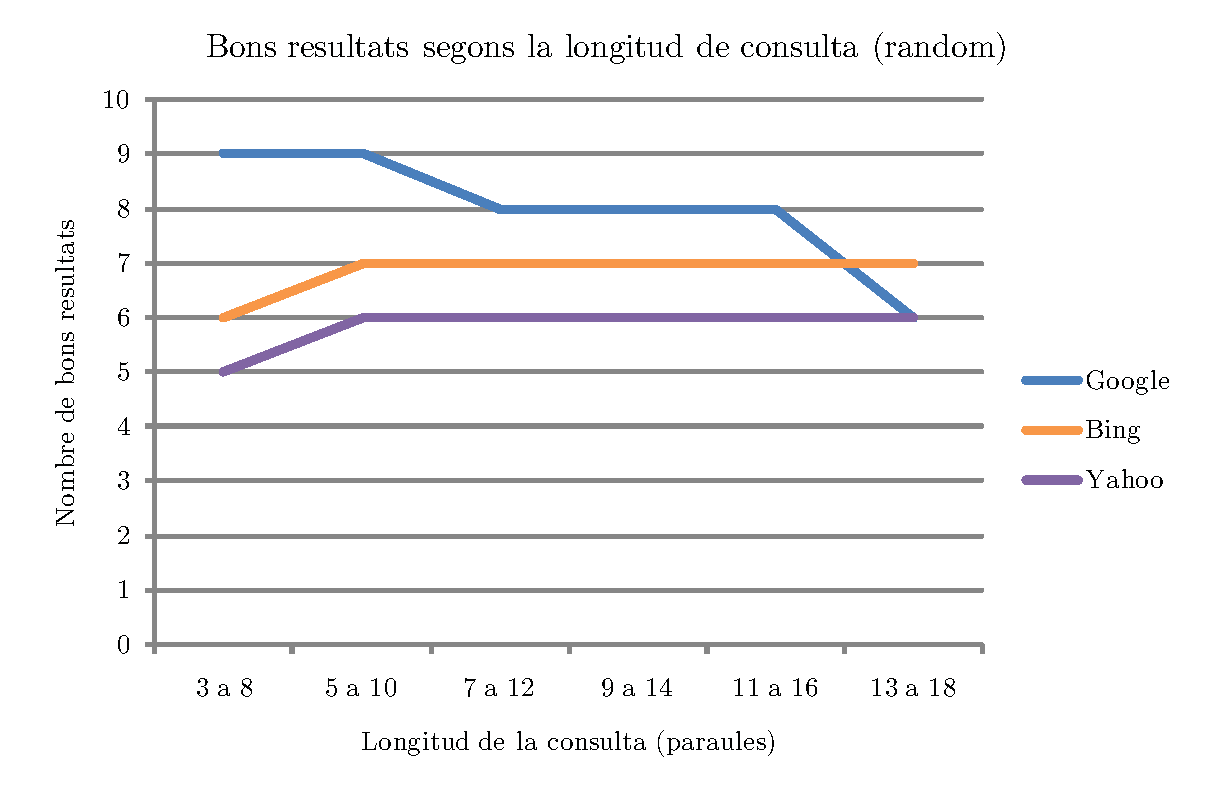
\includegraphics[width=0.9\textwidth]{figures/results:random-reslen.pdf}
\includegraphics[scale=0.8]{figures/results:search-legend.pdf}
\caption{Comparaci� de la qualitat dels resultats obtinguts segons la llargada de les consultes}
\label{fig:results:random-reslen}
\end{center}
\end{figure}

\paragraph{}
Tot i que en algunes ocasions els resultats bons retornats per \textit{Bing} o \textit{Yahoo} s�n superiors en nombre, en general, el cercador \textit{Google} ofereix major cobertura amb resultats sobre m�s articles.



\begin{figure}[!ht]
\begin{center}
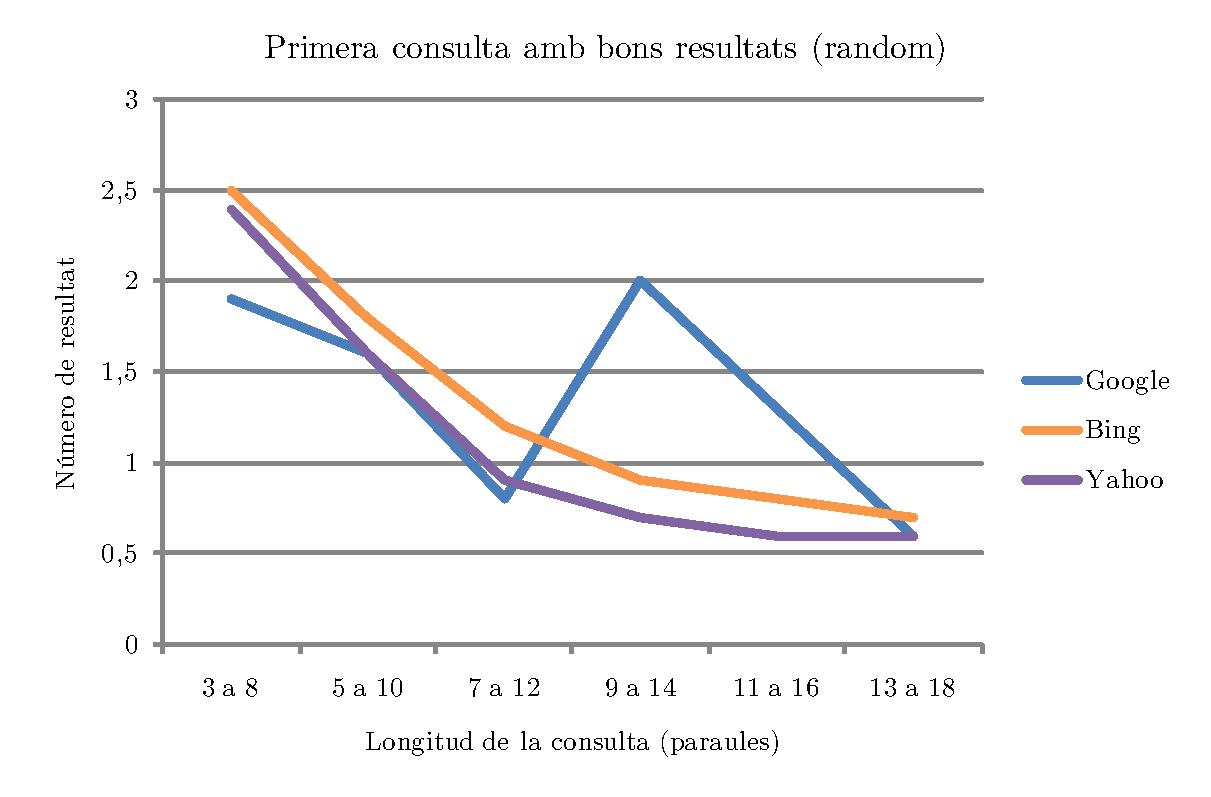
\includegraphics[width=0.9\textwidth]{figures/results:random-fqlen.pdf}
\includegraphics[scale=0.8]{figures/results:search-legend.pdf}
\caption{Comparaci� del n�mero de consultes necess�ries abans de trobar bons resultats}
\label{fig:results:random-fqlen}
\end{center}
\end{figure}

\paragraph{}
Finalment, respecte les consultes veiem que com mes llargues s�n, el n�mero de cerques que hem de fer per comen�ar a obtenir bons resultats disminueix. De totes maneres, tal i com ja s'ha dit a la secci� \ref{chapter:search:skip-queries}, per �s bo que ens saltem les primeres consultes per evitar cercar amb el t�tol de l'article.








%%%% WRAPPER INDUCTION %%%%
\section{Generaci� de \textit{wrappers}}
\label{chapter:results:section:wrapperinduction}
Per provar aquesta part del sistema, hem creat conjunts de p�gines web amb informaci� d'articles diferents i amb la refer�ncia corresponent. Les p�gines que inclou un grup corresponen totes a la mateixa biblioteca digital. Per cadascun d'aquests conjunts hem importat les refer�ncies i hem donat l'ordre al sistema de generar els \textit{wrappers} pels camps de cada biblioteca. Les mostres no s�n significatives, per� ens donen una idea per poder quantificar com de b� funciona l'aplicaci� dins l'entorn pel qual est� pensat.

\paragraph{}
Els resultats d'aquestes proves corresponen a les puntuacions rebudes durant l'avaluaci� dels \textit{wrappers} i que permeten marcar un ordre d'elecci� inicial a l'hora d'extreure refer�ncies. Com que de moment encara no hem fet proves amb p�gines que no s'han emprat per la generaci� (ho farem a la propera secci�), les gr�fiques no estan generats segons la correctesa dels resultats dels \textit{wrappers} sin� la \textit{confian�a} que tenim en que funcionin.

\paragraph{}
Hem classificat els \textit{wrappers} generats segons quatre grups de confian�a, depenent de la puntuaci� rebuda. La l�nia fosca correspon al percentatge de les biblioteques digitals per les quals hem obtingut almenys un \textit{wrapper} de confian�a m�xima. La l�nia clara indica el mateix percentatge, per� corresponent al seg�ent interval de confian�a. Els dos intervals m�s baixos s'han om�s.

\paragraph{}
Cal remarcar que el fet que per una biblioteca no s'hagi pogut obtenir un \textit{wrapper} que funcioni en tots els casos, no significa que no siguem capa�os d'extreure la informaci�. Tal i com hem vist a la secci� \ref{chapter:refextraction:section:fieldwrappers}, a l'hora d'extreure un camp, es prova m�s d'un \textit{wrapper}. Per tant, el que ens interessa m�s veure d'aquestes gr�fiques, �s la suma dels valors de les dues s�ries, que est� marcat amb una l�nia discontinua de gris molt clar.


\paragraph{}
Com ja s'ha comentat, els camps obligatoris que han de contenir les refer�ncies d'articles s�n: \textit{author}, \textit{title}, \textit{journal} i \textit{year}. A continuaci� es mostra la confian�a que tenim en els \textit{wrappers} per dos d'aquests camps, la informaci� sobre la resta es poden trobar a l'ap�ndix \ref{appendix:results:section:wrapperinduction}.

\begin{figure}[Ht]
\begin{center}
\includegraphics[width=0.8\textwidth]{figures/results:nwrappers-2.pdf}
\caption{Nombre de \textit{Wrappers} generats utilitzant 2 exemples i agrupats per confian�a}
\label{fig:results:nwrappers-2}
\end{center}
\end{figure}

\begin{figure}[Ht]
\begin{center}
\includegraphics[width=0.8\textwidth]{figures/results:nwrappers-4.pdf}
\caption{Nombre de \textit{Wrappers} generats utilitzant 4 exemples i agrupats per confian�a}
\label{fig:results:nwrappers-4}
\end{center}
\end{figure}

\begin{figure}[Ht]
\begin{center}
\includegraphics[width=0.8\textwidth]{figures/results:coverage-journal.pdf}
\caption{Cobertura dels \textit{wrappers} pel camp \textit{journal}}
\label{fig:results:coverage-journal}
\end{center}
\end{figure}

\begin{figure}[Ht]
\begin{center}
\includegraphics[width=0.8\textwidth]{figures/results:coverage-year.pdf}
\caption{Cobertura dels \textit{wrappers} pel camp \textit{year}}
\label{fig:results:coverage-year}
\end{center}
\end{figure}

\paragraph{}
El camp corresponent a l'any �s interessant perqu� moltes de les p�gines que hem provat contenen m�ltiples aparicions del valor que busquem, tot i que no sempre descriuen l'any de publicaci�, sin� la data de revisi�, la data a partir de la qual l'article es troba a Internet, \textit{copyright}, etc.
Aquest tipus de confusions tamb� s�n habituals en aquelles ocasions en qu�, a m�s de la informaci� de l'article, les p�gines inclouen el llistat d'articles als quals la publicaci� fa refer�ncia o b� la llista d'articles que el citen. Quan comencem a tenir exemples on aquests camps tenen valors diferents, al fer \textit{merging} de patrons s'acaben escollint els que s�n realment v�lids. 

\paragraph{}
Altres camps pels quals es t� m�s dificultat per generar \textit{wrappers} s�n aquells el valor dels quals consisteix en n�meros petits, com ara el n�mero de volum o de revista \textit{number}. El motiu �s el mateix, hi ha moltes aparicions del mateix valor, per� que no fan refer�ncia al camp que busquem.


%%%% REFERENCE EXTRACTION %%%%
\section{Extracci� de refer�ncies}
Anem a veure ara com de b� ho fan els \textit{wrappers} generats a la secci� anterior.

\paragraph{}
Recordem que nom�s s'aplicaran els \textit{field wrappers} generats si no hi ha cap \textit{reference wrapper} disponible o b� si no s'han obtingut resultats a l'aplicar-lo.

\begin{figure}[Ht]
\begin{center}
\includegraphics[width=0.8\textwidth]{figures/results:extraction-2.pdf}
\caption{Camps extrets amb els \textit{wrappers} generats amb 2 exemples}
\label{fig:results:extraction-2}
\end{center}
\end{figure}

\begin{figure}[Ht]
\begin{center}
\includegraphics[width=0.8\textwidth]{figures/results:extraction-4.pdf}
\caption{Camps extrets amb els \textit{wrappers} generats amb 4 exemples}
\label{fig:results:extraction-4}
\end{center}
\end{figure}

Pel que fa a al resta de camps que no es mostren als gr�fics, com ara el n�mero de volum, les p�gines, etc. els resultats s�n molt similars.

\begin{figure}[Ht]
\begin{center}
\includegraphics[width=0.8\textwidth]{figures/results:extraction-corrected.pdf}
\caption{Camps extrets per la biblioteca \textit{InformaWorld} despr�s de corregir els \textit{wrappers}}
\label{fig:results:extraction-4}
\end{center}
\end{figure}


\chapter{Conclusions i treball futur}
\label{chapter:conclusions}

Al llarg d'aquest document s'han descrit les decisions que hem pres i el proc�s seguit per poder implementar una aplicaci� d'extracci� de refer�ncies. Part�em d'aquest objectiu �nic i tot el que hem anat fent gira al voltant d'aquesta idea. Al final, hem comprovat que els resultats obtinguts s�n modestos.

Cal tenir en compte que, a cada pas, el proc�s es veu afectat per p�rdues inevitables:
\begin{itemize}
\item{}
L'extracci� del text dels fitxers PDF no es pot fer documents formats per imatges que han estat escanejats sense utilitzar \textit{software} de reconeixement de car�cters.
\item{}
El pas de cercar el document a Internet requereix, com �s l�gic, que es trobi en alguna de les biblioteques digitals indexades pels cercadors.
\item{}
Per �ltim, pel que fa a extreure informaci� de les p�gines HTML de forma correcta, ja hem vist que dep�n molt de les regles que tinguem definides, per� que els resultats tampoc no s�n perfectes.
\end{itemize}

Per aconseguir els objectius hem anat fent una s�rie d'assumpcions q...

Cal comentar que, tot i que el sistema est� destinat a l'extracci� de refer�ncies, la part de generaci� de regles i la manera d'aplicar-les podria ser, en realitat, la base d'un \textit{framework} �til per qualsevol altre sistema similar d'extracci� d'informaci� estructurada. En cas de no tractar-se de documents HTML, nom�s caldria afegir els nous tipus de regles necessaris.

Al ser un projecte \textit{open source}, qualsevol persona interessada es pot dirigir al repositori p�blic que hi ha al \textit{GitHub} i fer un \textit{fork} per continuar desenvolupant.

\section{Possibles Millores}
Objectivament, el sistema encara hauria de passar per m�s iteracions abans de poder-lo considerar s�lid. Alguns dels aspectes que s'haurien de tractar primer s�n:

\begin{itemize}
\item{}
El primer i m�s important seria incorporar millores a la generaci� d'expressi� regulars a partir d'exemples per tal d'aconseguir expressions generals utilitzant pocs exemples.
\item{}
Possibilitat d'actualitzar \textit{wrappers} a mesura que es disposa de nous exemples. Quan una refer�ncia s'extreu correctament de forma autom�tica significa que les regles funcionen, per� quan hi ha errors i l'usuari fa correccions, l'aplicaci� hauria de ser capa� d'adonar-sen i actualitzar lesl regles per fer-ho b� en pr�ximes execucions.
\item{}
Suportar altres llenguatges de citacions no nom�s suposaria poder importar i exportar refer�ncies amb aquests formats sin� que permetria que els \textit{reference wrappers} que hem descrit a la secci� \ref{refextraction:reference-wrappers} tamb� puguessin extreure aquest tipus refer�ncies.
\item{}
Millorar la interf�cie d'usuari; afegint funcionalitats, per� tamb� en termes d'usabilitat. Per exemple: caldria arreglar-la de manera que hi hagi consist�ncia en la manera de realitzar les mateixes operacions per totes les parts de l'aplicaci�.
\item{}
Tamb� referent a la interf�cie, seria convenient tenir opcions per poder configurar tots els par�metres de l'aplicaci� que actualment s'estableixen dins del fitxer de configuraci�.
\end{itemize}

Veiem, doncs, que encara queda molt per fer; tant com vulguem.


\bibliography{report}
\bibliographystyle{alpha}

\appendix{}
\chapter{Resultats dels tests}
\label{appendix-results}
A continuaci� es mostren els gr�fics amb la resta de resultats de les proves que s'han realitzat. La majoria corresponen al mateix tipus de tests que els del cap�tol \ref{chapter:results}, per� variant algun par�metre.

%%%% REF SEARCH %%%%
\section{Cerca de refer�ncies}
Les gr�fiques seg�ents s�n semblants a la de la figura \ref{fig:results:random-reslen}. En aquest cas, per�, el tipus de fitxers per als quals extraiem consultes i fem les cerques estan agrupats en dues categories segons l'estructura del seu contingut. Per un costat, a la figura \ref{fig:results:pageheader-reslen}, tenim fitxers que tenen una p�gina sencera com a cap�alera abans del resum o \textit{abstract} de l'article.
\begin{figure}[H]
\begin{center}
\includegraphics[width=0.8\textwidth]{figures/results:pageheader-reslen.pdf}
\includegraphics[scale=0.8]{figures/results:search-legend.pdf}
\caption{Qualitat dels resultats per fitxers amb una p�gina sencera com a cap�alera}
\label{fig:results:pageheader-reslen}
\end{center}
\end{figure}

Veiem que per aquest tipus d'article, el percentatge de p�gines per les quals s'han obtingut bons resultats disminueix molt a mesura que s'augmenta la llargada de la consulta. Cal tenir en compte que les consultes s'han obtingut totes a partir de la primera p�gina del fitxer. Al no contenir el resum, fa que l'expressi� regular usada per trobar la consulta no tingui coincid�ncies per la majoria dels articles provats. Si executem les mateixes proves, per� agafant les consultes de les dues primeres p�gines, els resultats milloren for�a:

\begin{figure}[H]
\begin{center}
\includegraphics[width=0.8\textwidth]{figures/results:pageheader2-reslen.pdf}
\includegraphics[scale=0.8]{figures/results:search-legend.pdf}
\caption{Qualitat dels resultats per fitxers amb una p�gina sencera com a cap�alera II}
\label{fig:results:pageheader2-reslen}
\end{center}
\end{figure}

El gr�fic de la figura seg�ent s'ha obtingut a partir d'articles que tenen una cap�alera \textit{normal}. Considerem que les cap�aleres dels articles m�s habituals s�n aquelles que tenen l'\textit{abstract} a la mateixa p�gina.
\begin{figure}[H]
\begin{center}
\includegraphics[width=0.8\textwidth]{figures/results:usualheader-reslen.pdf}
\includegraphics[scale=0.8]{figures/results:search-legend.pdf}
\caption{Qualitat dels resultats per fitxers amb cap�aleres \textit{normals}}
\label{fig:results:usualheader-reslen}
\end{center}
\end{figure}

\paragraph{}
Pel que fa al n�mero de consultes necess�ries per comen�ar a obtenir bons resultats, els gr�fics per aquests dos conjunts de fitxers s�n molt semblants al que hem vist a la figura \ref{fig:results:random-fqlen}.

%%% WRAPPER GEN %%%%
\section{Generaci� de \textit{wrappers}}
\label{appendix:results:section:wrapperinduction}
Pel que fa a la generaci� autom�tica de regles d'extracci�, la figura seg�ent mostra els \textit{wrappers} obtinguts al generar-los fent servir nom�s dos exemples. Com es pot comprovar, no se n'han generat tants com a l'utilitzar quatre exempes, per� tamb� hi ha \textit{wrappers} de confian�a m�xima per a la majoria de camps. Una altra cosa �s que realment funcionin a l'executar-los per nous documents, tal i com hem vist que passava.

\begin{figure}[H]
\begin{center}
\includegraphics[width=0.8\textwidth]{figures/results:nwrappers-2.pdf}
\caption{Nombre de \textit{Wrappers} generats utilitzant 2 exemples i agrupats per confian�a}
\label{fig:results:nwrappers-2}
\end{center}
\end{figure}

\paragraph{}
Tamb� hem mirat la \textit{cobertura} dels \textit{wrappers} generats per altres camps a part del nom de la revista i l'any. Els gr�fics de la figura \ref{fig:appendix:results:wrapperinduction:coverage} en mostren els resultats. �s interessant comparar la confian�a dels \textit{wrappers} d'autors, un camp multi-valor relativament dif�cil d'exterue; i la de les p�gines i el n�mero de volum. Els motius s�n els que ja s'han comentat a la secci� de resultats.

\paragraph{}
Per �ltim, tamb� hem generat un gr�fic (\ref{fig:appendix:results:wrapperinduction:time}) que reflecteix una mitjana del temps necessari per generar els \textit{wrappers} per un camp qualsevol depenent del n�mero d'exemples que s'utilitzen. 

\begin{figure}[H]
\begin{center}
\begin{minipage}{0.49\linewidth}
	\centering
	\includegraphics[width=\textwidth]{figures/results:coverage-title.pdf}
\end{minipage}
\hspace{0cm}
\begin{minipage}{0.49\linewidth}
	\centering
	\includegraphics[width=\textwidth]{figures/results:coverage-author.pdf}
\end{minipage}

\begin{minipage}{0.49\linewidth}
	\centering
	\includegraphics[width=\textwidth]{figures/results:coverage-pages.pdf}
\end{minipage}
\hspace{0cm}
\begin{minipage}{0.49\linewidth}
	\centering
	\includegraphics[width=\textwidth]{figures/results:coverage-volume.pdf}
\end{minipage}

\begin{minipage}{\linewidth}
	\centering
	
\includegraphics{figures/results:coverage-legend.pdf}
\end{minipage}

\caption{Cobertura dels \textit{wrappers} generats}
\label{fig:appendix:results:wrapperinduction:coverage}
\end{center}
\end{figure}



\begin{figure}[H]
\begin{center}
	\includegraphics[width=0.7\textwidth]{figures/results:field-time.pdf}
	\caption{Temps mitj� per la generaci� dels \textit{wrappers} d'un �nic camp}
	\label{fig:appendix:results:wrapperinduction:time}
\end{center}
\end{figure}
	



\chapter{Manual d'usuari}

L'aplicaci� es distribueix en forma d'\texttt{egg} de \textit{Python} i pot ser instal�lada de la manera est�ndard amb la comanda \texttt{easy\_install} (m�s detalls a \cite{pyEasyInstall}). Aquest cap�tol se centra a descriure alguns dels aspectes d'utilitzaci� de l'aplicaci� un cop instal�lada i mitjan�ant la interf�cie gr�fica. B�sicament, tindrem un men� amb dues grans categories: \textit{references} i \textit{wrappers}. Vegem qu� hi ha en cadascuna d'elles.

\section{Refer�ncies}

%%%% EXTRACT %%%%
\subsubsection{Extracci�}
La primera opci� del men� �s la que permet llegir un directori de fitxers PDF i obtenir-ne les refer�ncies. El sistema inclou \textit{wrappers} per les biblioteques digitals que s'han descrit en altres cap�tols d'aquest document, i per tant, des d'un principi ja es pot provar a fer extraccions d'articles indexats per aquestes biblioteques.
\\
\\
La vista de la figura \ref{fig:screenshots:extract-references} mostra el camp �nic que cal omplir per tal de comen�ar l'extracci�: simplement seleccionem un directori o fitxer i cliquem el bot� \textit{Extract References}. Durant l'execuci�, es mostra una barra de progr�s i una vegada finalitzat, se'ns mostrar� una finestra molt semblant a la de la figura \ref{fig:screenshots:import-references-2} indicant-nos que podem veure i editar les refer�ncies amb l'opci� del men� \textit{Manage}.
\begin{figure}[ht]
\begin{center}
\includegraphics[width=0.9\textwidth]{figures/screenshots/screenshots:extract-references.pdf}
\caption{Extreu refer�ncies}
\label{fig:screenshots:extract-references}
\end{center}
\end{figure}

%%%% MANAGE %%%%
\subsubsection{Gesti�}
Amb l'opci� \textit{Manage} (veure \ref{fig:screenshots:manage-references}) podrem gestionar les refer�ncies disponibles i realitzar les operacions CRUD t�piques. A la part esquerra es mostra un llistat de totes les refer�ncies de la base de dades. Al seleccionar-ne una s'omplir� l'editor de la meitat dreta de la finestra amb tota la informaci� sobre la refer�ncia.

\begin{figure}[ht]
\begin{center}
\includegraphics[width=0.9\textwidth]{figures/screenshots/screenshots:manage-references.pdf}
\caption{Maneig de refer�ncies}
\label{fig:screenshots:manage-references}
\end{center}
\end{figure}

Algunes caracter�stiques:
\begin{itemize}
\item{}
Podem crear nous camps, autors i editors simplement afegint-los al final de la llista adequada, a la l�nia buida que hi ha. Per eliminar-los, nom�s cal esborrar totes les columnes i deixar la fila en blanc.
\item{}
Per afegir o eliminar noves refer�ncies podem fer-ho a partir del men� contextual que apareix al clicar amb el bot� secundari sobre la llista \textit{Available References}.
\item{}
�s necessari definir una URL com a valor del camp \textit{Extracted from} si posteriorment es pret�n utilitzar la refer�ncia en q�esti� per generar \textit{wrappers}.
\item{}
Pel que fa al camp \textit{File Path}, nom�s serveix per ajudar a l'usuari a distingir entre les m�ltiples refer�ncies disponibles de la llista \textit{Available References}.
\end{itemize}

%%%% IMPORT %%%%
\subsubsection{Importaci�}
\begin{figure}[ht]
\begin{center}
\includegraphics[width=0.9\textwidth]{figures/screenshots/screenshots:import-references.pdf}
\caption{Importa refer�ncies}
\label{fig:screenshots:import-references}
\end{center}
\end{figure}
Aquesta opci� �s la que probablement m�s ens interessar� la primera vegada que executem l'aplicaci� just despr�s d'instal�larla. Permet importar refer�ncies des de fitxers \texttt{.bib} de manera que sigui ben f�cil comen�ar a generar \textit{wrappers} i configurar el sistema segons les necessitats de cadasc�. El funcionament �s molt semblant al de les extraccions. Se selecciona un fitxer a la finestra \ref{fig:screenshots:import-references} i un cop s'ha acabat, se'ns re-dirigir� a la vista de la figura \ref{fig:screenshots:import-references-2}.


\begin{figure}[ht]
\begin{center}
\includegraphics[width=0.9\textwidth]{figures/screenshots/screenshots:import-references-2.pdf}
\caption{Un cop s'han importat les refer�ncies}
\label{fig:screenshots:import-references-2}
\end{center}
\end{figure}

%%%% EXPORT %%%%
\subsubsection{Exportaci�}
La darrera opci� que queda relacionada amb les refer�ncies �s la funcionalitat que permet exportar-les en format \BibTeX{}. De la mateixa manera que amb la finestra \textit{Manage}, a la part esquerra se'ns llistaran totes les refer�ncies disponibles. Podrem seleccionar les que vulguem i la seva entrada formatada apareixer� a l'�rea de text de la part dreta. Hi ha la possibilitat de seleccionar o b� des-seleccionar tots els elements de la llista a partir del men� contextual que apareix al fer clic amb el bot� secundari.
Tamb� podem desar totes les entrades seleccionades directament a un fitxer amb el bot� \textit{Save to file}.

\begin{figure}[ht]
\begin{center}
\includegraphics[width=0.9\textwidth]{figures/screenshots/screenshots:export-references.pdf}
\caption{Exporta refer�ncies}
\label{fig:screenshots:export-references}
\end{center}
\end{figure}


%%%% WRAPPERS %%%%
\clearpage
\section{\textit{Wrappers}}
L'altra categoria �s la que permet gestionar els \textit{wrappers}. 


%%%% TRAIN %%%%
\subsubsection{Entrenament}
Aquesta opci� �s la que ens permet generar nous \textit{wrappers} a partir de les refer�ncies de les que es disposa. La vista que permet executar aquesta funcionalitat �s la de la figura \ref{fig:screenshots:wrapper-train}. Les URLs de les biblioteques per les quals ja s'han generat \textit{wrappers} amb anterioritat es mostren a la llista \textit{Available URLs}, facilitant el re-entrenament un cop les dades deixen d'extreure's correctament. En el cas que es tracti d'una biblioteca nova, podem introduir-ne la seva adre�a (o un prefix) manualment al camp \textit{URL}.
\\
\\
Un cop hem escollit la biblioteca, nom�s hem de clicar el bot� \textit{Train} i deixar que l'aplicaci� faci la resta. Quan finalitza, es mostra un missatge indicant que podem veure i editar els \textit{wrappers} generats des amb l'opci� \textit{Manage}.

\begin{figure}[ht]
\begin{center}
\includegraphics[width=0.9\textwidth]{figures/screenshots/screenshots:wrapper-train.pdf}
\caption{Entrenament de \textit{wrappers}}
\label{fig:screenshots:wrapper-train}
\end{center}
\end{figure}


%%%% MANAGE %%%%
\subsubsection{Gesti�}
De la mateixa manera que podem modificar les refer�ncies, tamb� tenim un editor pels \textit{wrappers} generats; es mostra a la finestra de la figura \ref{fig:screenshots:wrapper-manager}. En aquest cas tenim tres apartats:
\begin{itemize}
\item{}
Llistat de col�leccions de \textit{wrappers} agrupades segons la biblioteca digital a la qual corresponen.
\item{}
Llistat de \textit{wrappers} de la col�lecci� seleccionada en un moment donat. Per cadascun d'ells es mostra la puntuaci� rebuda.
\item{}
Editor del \textit{wrapper} seleccionat a la llista anterior. Es mostren els vots positius, negatius, la puntuaci� calculada i el llistat de regles.
\end{itemize}

Podem crear i eliminar regles afegint nous valors a la l�nia buida que hi ha al final de la llista \textit{Rules} i deixant l�nies en blanc, respectivament. Les col�leccions i els \textit{wrappers} es poden crear i esborrar amb el men� contextual que apareix al clicar amb el bot� secundari. Aquesta inconsist�ncia a l'hora de realitzar la mateixa operaci� per elements diferents �s un problema que caldr� solucionar en un futur.

\begin{figure}[ht]
\begin{center}
\includegraphics[width=0.9\textwidth]{figures/screenshots/screenshots:wrapper-manager.pdf}
\caption{Gesti� de \textit{wrappers}}
\label{fig:screenshots:wrapper-manager}
\end{center}
\end{figure}





\chapter{Biblioteques utilitzades}
A continuaci� es llisten les diferents biblioteques i m�dules \textit{Python} que s'han utilitzat en l'aplicaci�

\begin{itemize}
\item{SimpleJSON}
\item{DiffLib}
\item{}
\end{itemize}

\chapter{Diagrames}
\label{appendix:diagrams}
En aquest ap�ndix es mostren alguns diagrames que poden ajudar a entendre una mica millor l'aplicaci�. Creiem que cada diagrama �s autoexplicatiu nom�s s'acompanyen d'una petita descripci� als peus de cadascun d'ells.

\begin{figure}[H]
\begin{center}
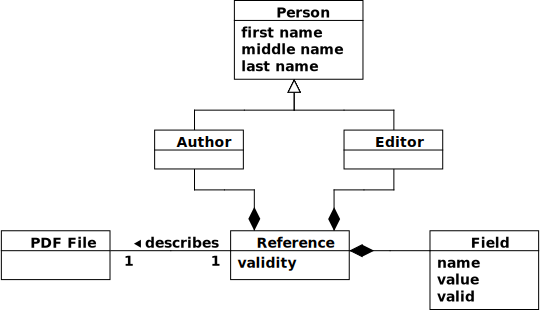
\includegraphics[width=0.7\textwidth]{figures/diagrams:references-domain-model.pdf}
\caption{Model de domini respecte a refer�ncies}
\label{fig:diagrams:references-domain-model}
\end{center}
\end{figure}


\begin{figure}[H]
\begin{center}
\includegraphics[width=0.7\textwidth]{figures/diagrams:wrappers-domain-model.pdf}
\caption{Model de domini dels \textit{wrappers}}
\label{fig:diagrams:wrappers-domain-model}
\end{center}
\end{figure}

\begin{figure}[H]
\begin{center}
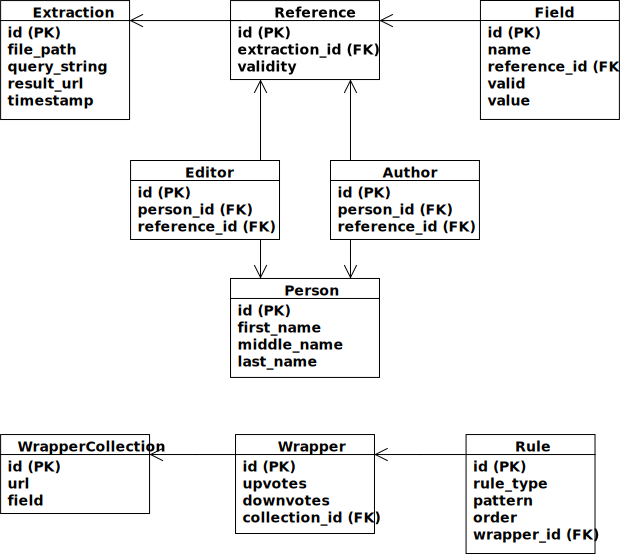
\includegraphics[width=0.8\textwidth]{figures/diagrams:database-diagram.pdf}
\caption{Estructura de la base de dades}
\label{fig:diagrams:database-diagram}
\end{center}
\end{figure}


\begin{figure}[ht]
\begin{center}
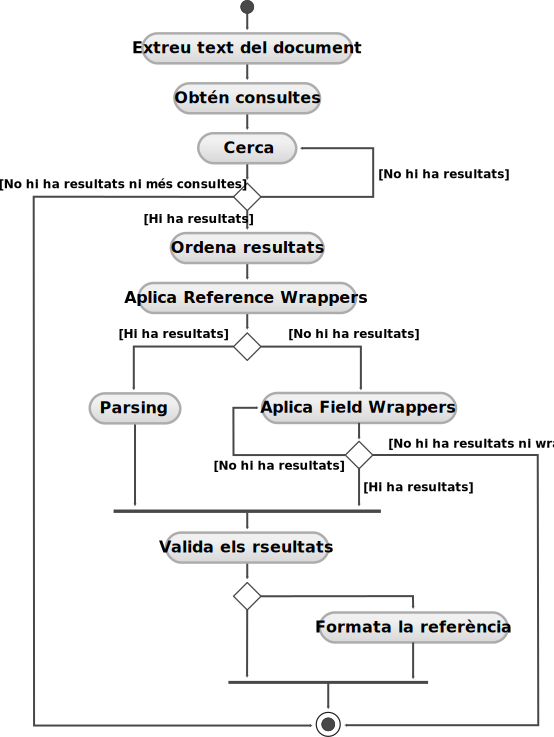
\includegraphics[width=0.95\textwidth]{figures/diagrams:extraction-activity.pdf}
\caption{Diagrama d'activitat per a l'extracci� de refer�ncies}
\label{fig:diagrams:extraction-activity}
\end{center}
\end{figure}

\clearpage





\chapter{Extracci� Contingut PDF}
\label{appendix-pdf2text}

\chapter{Biblioteques digitals}
Al llarg d'aquest document hem definit qu� s�n les biblioteques digitals i tamb� n'hem anat esmentant algunes de les que hi ha disponibles a Internet. En aquest ap�ndix nom�s intentem llistar i facilitar enlla�os a totes les que s'han utilitzat a l'hora de realitzar les proves. Com a curiositat, tamb� hem incl�s petites introduccions extretes de les descripcions escrites per ells mateixos:

\begin{itemize}
\item{ACM Portal:}\textit{
Full text collection of every article published by ACM, including over 50 years of archives.
}
\\
\url{http://portal.acm.org}



\item{CiteSeerX:}\textit{
is a scientific literature digital library and search engine that focuses primarily on the literature in computer and information science. 
}
\\
\url{http://citeseerx.ist.psu.edu}



\item{CiteULike:}\textit{
is a free service for managing and discovering scholarly references.
}
\\
\url{http://www.citeulike.org}



\item{EconPapers:}\textit{
EconPapers use the RePEc bibliographic and author data, providing access to the largest collection of online Economics working papers and journal articles.
}
\\
\url{http://econpapers.repec.org}



\item{IDEAS:}\textit{
is a service providing information about working papers and published research to the economics profession. IDEAS stands for ``Internet Documents in Economics Access Service'', which is not very good English, but you get the idea... 
}
\\
\url{http://ideas.repec.org}



\item{IEEE Computer Society:}\textit{
With nearly 85,000 members, the IEEE Computer Society is the world's leading organization of computing professionals. [...] the Computer Society is dedicated to advancing the theory and application of computing and information technology.
}
\\
\url{http://www.computer.org}



\item{Informa World:}\textit{
is the leading provider of specialist information to the global academic \& scientific, professional and commercial communities via publishing, events and performance improvement.
}
\\
\url{http://www.informaworld.com}



\item{ScientificCommons:}\textit{
aims to provide the most comprehensive and freely available access to scientific knowledge on the internet. The major aim of the project is to develop the world's largest communication medium for scientific knowledge products which is freely accessible to the public.
}
\\
\url{http://en.scientificcommons.org}



\item{ScienceDirect:}\textit{
is a leading full-text scientific database offering journal articles and book chapters from more than 2,500 peer-reviewed journals and more than 11,000 books.
}
\\
\url{http://www.sciencedirect.com}



\item{SpringerLink:}\textit{
One of the world's leading interactive databases for high-quality STM journals, book series, books, reference works and the Online Archives Collection. SpringerLink is a powerful central access point for researchers and scientists.
}
\\
\url{http://springerlink.com}
\end{itemize}



\input{blank}
\input{blank}
\input{blank}
\input{blank}
\end{document}
